\documentclass{article}

\usepackage{geometry}
\usepackage{algorithm}
\usepackage{algpseudocode}
\usepackage{graphicx}
\geometry{a4paper, total={5.5in, 8.5in}}

\algrenewcommand{\algorithmiccomment}[1]{\{#1\}}
\algrenewcommand\algorithmicuntil{}
\renewcommand\tablename{Tabelul}
\renewcommand\figurename{Figura}

\begin{document}

Presupunem, pentru simplificare, că vârfurile sunt numerotate, $V=\{1, 2, \ldots, n\}$, vârful 1 fiind sursa, şi că matricea $L$ dă lungimea fiecărei muchii, cu $L[i,j] = +\infty$ dacă muchia $(i, j)$ nu există. Soluţia se va construi în tabloul $D[2 .. n]$. Algoritmul este:

\begin{algorithmic}
\Function{Dijkstra}{$L[1 .. n, 1 .. n]$}
	\State \Comment{iniţializare}
	\State $C \gets \{2, 3, \ldots, n\}$ \qquad \Comment{$S = V \setminus C$ există doar implicit}


	\For{$i \gets 2$ \textbf{to} $n$}
		\State $D[i] \gets L[1,i]$
	\EndFor

	\State \{bucla greedy\}

	\Repeat $\;n-2$ \textbf{times}
		\State $v \gets$ vârful din $C$ care minimizează $D[v]$
		\State $C \gets C \setminus \{v\}$ \qquad \Comment{şi, implicit, $S \gets S \cup \{v\}$}
		\For{fiecare $w \in C$}
			\State $D[w] \gets$ min$(D[w], D[v] + L[v,w])$
		\EndFor
	\Until{}
	\hspace{-.1cm}\Return{$D$}
\EndFunction
\end{algorithmic}

Pentru graful din Figura \ref{fig:graf}, paşii algoritmului sunt prezentaţi în Tabelul \ref{tbl:algo}.


Observăm că $D$ nu se schimbă dacă mai efectuăm o iteraţie pentru a-l scoate şi pe $\{2\}$ din $C$. De aceea, bucla greedy se repetă doar de $n-2$ ori.

Se poate demonstra următoarea proprietate:

\begin{figure}[htbp]
	\centering
	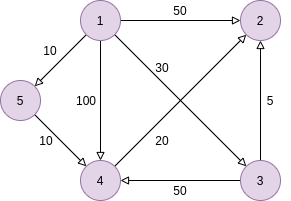
\includegraphics[scale=.7]{graf.png}

	\caption{Un graf orientat} \label{fig:graf}
\end{figure}

\begin{table}[htbp]
	\centering
	
	\begin{tabular}{c c l l}
		\textbf{Pasul} & $v$ & \multicolumn{1}{c}{$C$} & \multicolumn{1}{c}{$D$} \tabularnewline
		iniţializare & $—$ & $\{2,3,4,5\}$ & $[50,30,100,10]$\\
		1 & $5$ & $\{2,3,4\}$ & $[50,30,20,10]$\\
		2 & $4$ & $\{2,3\}$ & $[40,30,20,10]$\\
		3 & $3$ & $\{2\}$ & $[35,30,20,10]$\\
	\end{tabular}

	\caption{Algoritmul lui Dijkstra aplicat grafului din Figura \ref{fig:graf}} \label{tbl:algo}
\end{table}

\end{document}
